% Please keep it to 80 columns, no tabs, no trailing whitespace
% and no Windows line endings (\r\n)
\documentclass[10pt,a4paper,oneside]{report}
\usepackage[paper=A4,pagesize]{typearea}
\usepackage{afterpage}
\usepackage[utf8]{inputenc}
\usepackage{geometry}
\usepackage{graphicx}
\usepackage{lscape}
\usepackage{float}
\usepackage{pdfpages}
\usepackage{graphics}
\usepackage{enumitem}
\usepackage{tabularx}
\begin{document}
\title{Group 8 Integrated Project Proposal}

% Names in alphabetical order.
\author{
  Chen Guangyu (20\%)\\
  Kowalczyk Mateusz (20\%)\\
  Luff Katie (20\%)\\
  Sampson Robert (20\%)\\
  Singh Aman (20\%)\\ }
\maketitle
\section*{Abstract}
In this submission we gathered the requirements of our map application and created a detailed report of the requirement analysis. We then created sketches of the user interface and made use case scenarios that depicted interactions between the user and the application. Finally we described the architectural design and the implementation environment of the application.

The main requirements include viewing the current location, finding any location, landmark or computer rooms on campus. We added these features to help freshers and newcomers at the university to easily locate landmarks.

For planning and management we first categorised the task into 4 phases, System Requirements, Architectural Design and Sketches, System prototype implementation and System Test Planning.  We then split up our group into 2 sub-groups each performing 2 of the sub-tasks.
We decided that the requirement gathering process would be done before the architectural design so that the design team would have complete knowledge about all the features of the application.
We also made sure that the team that did the requirements created the test plan since they would exactly know which feature functionality has to be tested.
\section*{Introduction}
This document contains an introduction and specification of the four main stages our interactive map application. These are, gathering system requirements, specifying the architectural design, implementing a prototype and creating test cases for the system.
The Software Process Model that we have chosen for this application is the incremental and iterative model. The reason for choosing the incremental model is that this model allows us to focus and develop core features first and then add on other features in small easy to test increments. Since our model has one core feature which is finding locations by implementing shortest path finder algorithms, this model is the most suitable. We have also decided to progress with the project in an iterative way because several ideas may be developed throughout the lifetime of the development (e.g... bus finder, bus timetable, lecture timetable features).  An iterative model will allow these new ideas (future requirements) to develop in forthcoming iterations.
\begin{figure}[H]
 \centering
 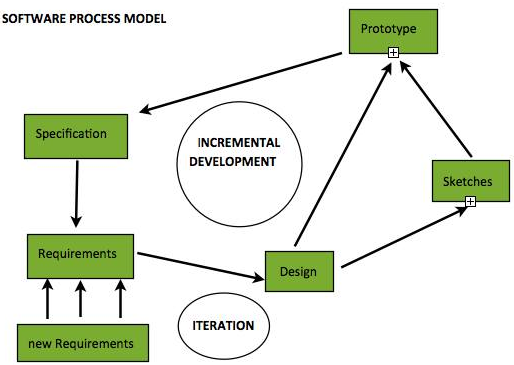
\includegraphics[keepaspectratio, width=\textwidth]{spm.png}
\end{figure}

\section*{Requirements}
\subsection*{Context of Application}
\subsubsection*{Application type}
 The application is an interactive map of the university of bath. This map will help students and new comers at the university to find major buildings, landmarks, eateries as well as free computer rooms on campus. This application will help students save a lot of time as well as enhance their university experience.

\subsubsection*{Problem domain}
The problem domain is the complexity of the application. The application developers have to make a compromise between having several features versus keeping the application plain and simple with only a few core features.

\subsubsection*{Solution offered}
The solution offered is somewhere in between both extremes. The app is simple as it offers 3 core features: finding landmarks, finding computers, sharing location/events.
The application also has other small features: get information about the landmark, get a person’s location, save favourite destinations...
\subsection*{Establishing the requirements}
The requirements were established by our own domain knowledge and by the help of a survey.
We were fresher’s last year and wasted a lot of time finding lecture halls and other buildings on campus. The computers in the library were full during peak hours and our lack of knowledge of the location of free computer rooms meant that we had to travel back home to work. Thus, it was our personal experience that led to the establishment of the core requirements. The rest of the requirements were gathered using a survey. \\

\textbf{Katie, your Survey will go here}
\clearpage

\subsection*{Ethics}
Our application involves holding the information regarding the location of individual as well as other personal information. We have decided to have security measures to prevent unauthorised access to the personal information of every user. The application also allows each user to share his current location with only a private group of friends/acquaintances; we will provide sufficient encryption to ensure that only the tagged friends can access this location. For extra security we have decided to allow each user to share his location for only 10 minutes after which the location will disappear from the map.

\subsection*{User domain}
The users of this application are fresher’s and visitors  to the university.  The fresher’s signify the “professional” users of the application who will use all the features. The other users are the “short term” users who will basically use the core features, such as the find location/landmark feature.

\subsection*{Functional requirements}
\small{
\begin{enumerate}
\item{The application must allow a user to view his/her current location on the map. \\
  \textbf{Rationale}: This will allow new comers to know their exact location on the map.\\
  \textbf{Success criteria}: upon request, the user should be notified about his current location on the map. This should be done by marking his current location with a marker/ pin.\\
  \textbf{Priority}: 1\\
  \textbf{Source}: domain knowledge.\\
}
\item{The application must allow a user to share his/her current location with all his contacts. \\
  \textbf{Rationale}: This will allow the users to find each other on campus.\\
  \textbf{Success criteria}: upon request, the user should be able to broadcast his location as an event which will be received by users who are currently logged on to the system.\\
  \textbf{Priority}: 2\\
  \textbf{Source}: domain knowledge
}
\item{The application will allow the users to view all rooms on campus with free computers. In addition, it will also suggest the closest room among these. \\
  \textbf{Rationale}: students waste time finding free computers during peak hours. Such a function would allow them to view free computer rooms as well as help them to find the closest ones from their current locations.\\
  \textbf{Success criteria}: upon request. The user should be able to view all rooms with free computers as well as find the path to the closest room.\\
  \textbf{Priority}: 1\\
  \textbf{Source}: survey.
}
\item{The application will allow users to find lecture halls, eateries, shops and other landmarks by providing them will the shortest route from their current location to their destinations. \\
  \textbf{Rationale}: new comers to the university often find it hard to find locations on campus\\
  \textbf{Success criteria}: upon request, the user should be able to enter his/her destination. The\\
  \textbf{Applications} should then provide the user with the shortest route to the destination.\\
  \textbf{Priority}: 1.\\
  \textbf{Source}: survey
}
\item{The application will allow users to share event locations on campus. \\
  \textbf{Rationale}: This will allow users to plan social gatherings/parties and display the location on the map.\\
  \textbf{Success criteria}: upon request, the user should be able to arrange an event and mark it on the map which will be received by users who are currently logged on to the system.\\
  \textbf{Priority}: 3\\
  \textbf{Source}: Survey
}

\item{The application will inform the users about weather and climatic conditions. The UI of the system will change according to the weather.\\
  \textbf{Rationale}: The weather in Bath is unpredictable and such a feature would inform users about the weather conditions in real time. The changing UI will make the application more intuitive and fun to use.\\
  \textbf{Success Criteria}: upon request, the user should be notified about the weather conditions in real time. The UI should automatically change according to the current climatic conditions.\\
  \textbf{Priority}: 3\\
  \textbf{Source}: Survey
}

\item{The application will allow users to save their favourite destinations in a list.\\
  \textbf{Rationale}: This will provide to the user a list of top destinations (coffee shop etc.) visited in the past.\\
  \textbf{Success Criteria}: upon request, the user should be able to view a list of favourite destinations stored by the user.\\
  \textbf{Priority}: 3\\
  \textbf{Source}: Survey
}

\item{The application will allow users to get the precise location of their friends on campus.\\
  \textbf{Rationale}: Such a feature will allow users to find their friends on campus.\\
  \textbf{Success Criteria}: upon request, the application will provide the exact location of the friend via a pop up widget (pin).\\
  \textbf{Priority}: 3\\
  \textbf{Source}: Survey
}

\item{The application will provide users with useful  information regarding a particular selected landmark. (Example: timings of a coffee shop)\\
  \textbf{Rationale}: Such a feature would provide information such as opening and closing timings of buildings, this would save them valuable time.\\
  \textbf{Success Criteria}: upon request, the application will display information about the selected landmark.\\
  \textbf{Priority}: 3\\
  \textbf{Source}: Survey
}
\end{enumerate}
}
\subsection*{Non-functional requirements}
\small{
\begin{enumerate}
  \item{Usability}
    \begin{enumerate}[label*=\arabic*.]
      \item{The application must have an intuitive interface, which is simple and easy to navigate.}
        \begin{enumerate}[label*=\arabic*.]
          \item{The user interface must have a simple layout and colour scheme in order to let the interface flow easily.}
          \item{The user interface should be designed so that everything is very self-explanatory and thus no user training is required.}
        \end{enumerate}
    \end{enumerate}

    \item{Efficiency}
      \begin{enumerate}[label*=\arabic*.]
      \item{The application must be fast and responsive.}
        \begin{enumerate}[label*=\arabic*.]
        \item{The application must open in under 1s on average.}
          \begin{enumerate}[label*=\arabic*.]
          \item{The application must have fully loaded, and be usable in under 3s on average.}
          \end{enumerate}
        \item{All page transitions in the Application must be completed in less than 500ms.}
          \begin{enumerate}[label*=\arabic*.]
          \item{The application must take no longer than 5 seconds to find a route once the co-ordinates of the user have been established}
          \end{enumerate}
        \end{enumerate}
      \item{The application must have a small footprint on the system’s memory and disk space.}
        \begin{enumerate}[label*=\arabic*.]
        \item{The application (exclusive of the user’s data) must not be larger than 100MBs.}
        \item{The application must not use more than 50MBs of RAM.}
        \end{enumerate}
      \end{enumerate}

    \item{Reliability}
      \begin{enumerate}[label*=\arabic*.]
      \item{The application must save all data after a forced closure.}
      \item{The application must not lose any data inputted to the system.}
        \begin{enumerate}[label*=\arabic*.]
        \item{The data must not corrupt in any way.}
        \end{enumerate}
      \end{enumerate}


    \item{Delivery}
      \begin{enumerate}[label*=\arabic*.]
      \item{The application must be deliverable through an existing mobile application market place.}
        \begin{enumerate}[label*=\arabic*.]
        \item{The download must be kept smaller than 100MBs.}
        \end{enumerate}
      \end{enumerate}

    \item{Compatibility}
      \begin{enumerate}[label*=\arabic*.]
      \item{The application must be compatible with all devices able to download the application.}
        \begin{enumerate}[label*=\arabic*.]
        \item{The application should be able to download on all current Android versions since 4.2.}
        \end{enumerate}
      \item{The application must be compatible with the mobile phone’s GPS navigation system.}
      \end{enumerate}

    \item{Ethical}
      \begin{enumerate}[label*=\arabic*.]
      \item{The application must not perform any kind of computation on the personal data held within the application without the user’s permission.}
      \item{The application must not transmit any of the user’s personal information.}
        \begin{enumerate}[label*=\arabic*.]
        \item{The application must not display the user’s location, unless the user has specifically allowed it to do so.}
        \end{enumerate}
      \end{enumerate}
\end{enumerate}
}

\subsection*{Managing requirement conflicts}
The requirements were thoroughly examined to see whether any requirements were conflicting. None were found. For future requirements that may conflict, the requirement having a higher priority will take precedence. For requirements having the same priority several approaches can be taken. We can either construct the requirements again, or take a survey, or just have a vote within the group for which requirement will be selected.

\begin{figure}[H]
 \centering
 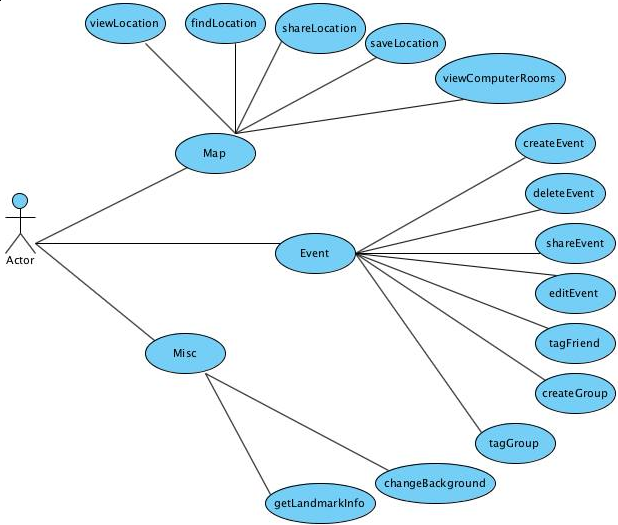
\includegraphics[keepaspectratio, width=\textwidth]{usecase.png}
 \caption{Use case diagram}
\end{figure}

\section*{Architectural design}
\subsection*{Control style}
The application will run on an Android mobile device. The design style should be such that it should respond efficiently to the users touch input.  Once in the home menu the user can select any number of set interactive objects which will dispatch an event handler. Since we precisely know the number of events to be handled the best control style is an Event Driven System.

\begin{figure}[H]
 \centering
 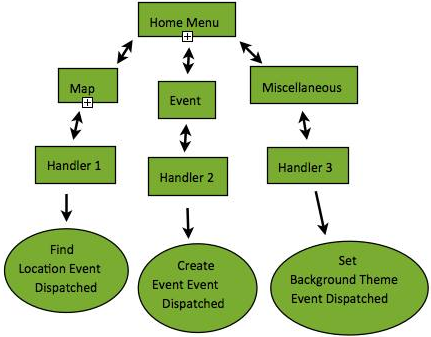
\includegraphics[keepaspectratio, width=\textwidth]{event.png}
 \caption{Interactive application event-driven system}
\end{figure}

\subsection*{Application architecture}
Our application will follow the client-server model out of necessity. While the basic application use requires no communication with the network, features such as location and event sharing do. As there are no means of easily discovering and communicating with users of the application, user's device will instead connect to the server and communicate with others through there. The sole purpose of the server will be to forward information requests. As we're going to be using public key cryptography to exchange information about events and user locations, initial public key swap is also going to be done through the server. As all other communication will be encrypted, the server is kept in the dark about what locations and events are being transferred. This grants high user privacy and frees us from the burden of taking high security measures ourselves to protect sensitive user data.

\subsection*{Sequence diagrams}

\begin{figure}[H]
 \centering
 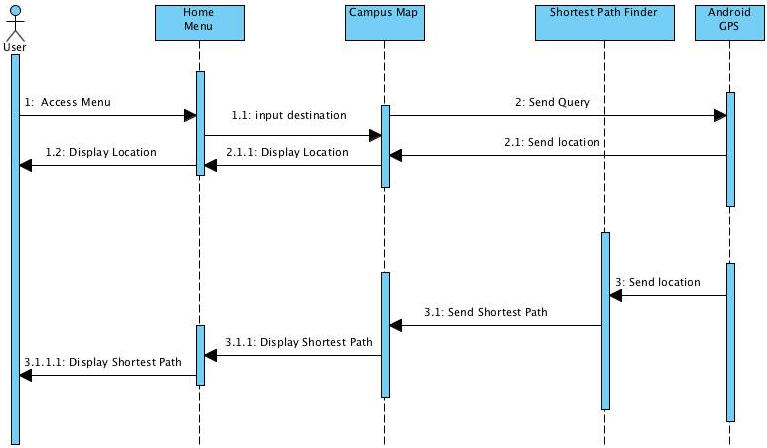
\includegraphics[keepaspectratio, scale=0.5]{seqfind.png}
 \caption{Finding a location on campus}
\end{figure}
\subsubsection*{Initial status}
The user already logs on the application and he is accessing the main menu
\subsubsection*{Normal action}
The user reaches the main menu and clicks “Find location” button. Then there’s a list of possible locations for the user to choose from. The user chooses a particular destination he wants to go. From there the system gets the corresponding choice and send it to the map component, the map component send the query to the android GPS module. The GPS will send the coordinate of the location and mark it on the map. In addition the user can get information on the shortest route to the destination from Android GPS.
\subsubsection*{Possibilities of failure}
The system may provide inaccurate position information to the user. The GPS may calculate an unnecessary path to the destination. The user may choose a destination within the deviation of the GPS and this will result in incorrect navigation.
\subsubsection*{Complete state}
A pin-shape mark of the destination is displayed on the map. A highlighted path is also displayed on the map connecting the user’s current location to the destination.

\begin{figure}[H]
 \centering
 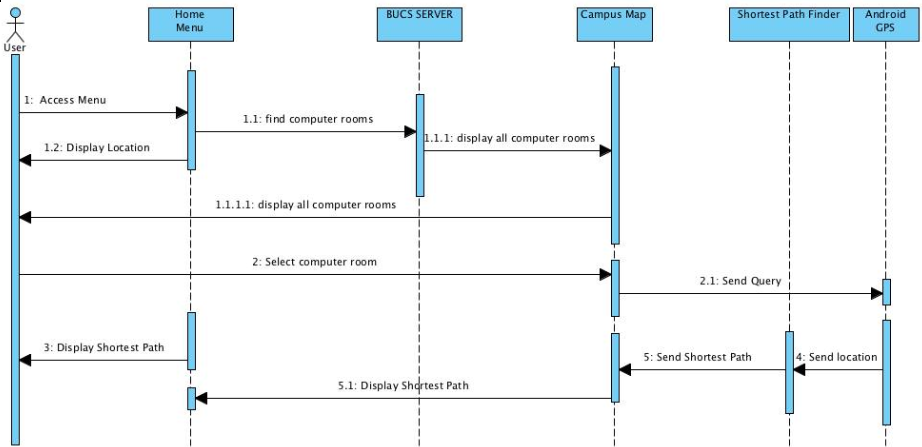
\includegraphics[keepaspectratio, scale=0.5]{seqcomp.png}
 \caption{Finding a computer room}
\end{figure}

\subsubsection*{Initial status}
The user already logs on the application and he is accessing the main menu
\subsubsection*{Normal action}
The user reaches the main menu and clicks the button “find computers”. The system send query to the BUCS website with information regarding rooms of free computers available in real time. Then the system returns the message and shows all the locations of the rooms of free computers on the campus map according to the website. The user then chooses a location among these choices. The system sends the information regarding user’s choice. The GPS module calculates the shortest path to the location and returns this message to the user.
\subsubsection*{Possibilities of failure}
The BUCS website may not provide accurate and real time information about the rooms with free computers. There’s a possibility that the computers in a room may have already been taken up before the information is updated to BUCS website.
\subsubsection*{Complete state}
The user is shown the positions of the rooms with free computers on the map. In addition, a shortest path to the chosen destination is also showed on the map.

\begin{figure}[H]
 \centering
 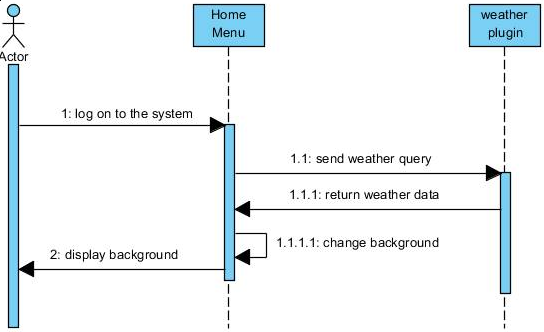
\includegraphics[keepaspectratio, scale=0.5]{seqback.png}
 \caption{Application background change}
\end{figure}

\subsubsection*{Initial state}
The user switches on the application. The main menu and background is showed.
\subsubsection*{Normal action}
As soon as the user logs on the system, the system sends a query regarding the weather conditions. Then the weather plug-in returns the message with real-time weather condition of the nearby area. The main menu changes the background according to the message given.
\subsubsection*{Possibilities of failure}
In normal cases, if the device has consistent internet connection. The system will behave what it supposed to be.
\subsubsection*{Complete state}
The user will see the menu background with the image of the latest updated weather condition.

\begin{figure}[H]
 \centering
 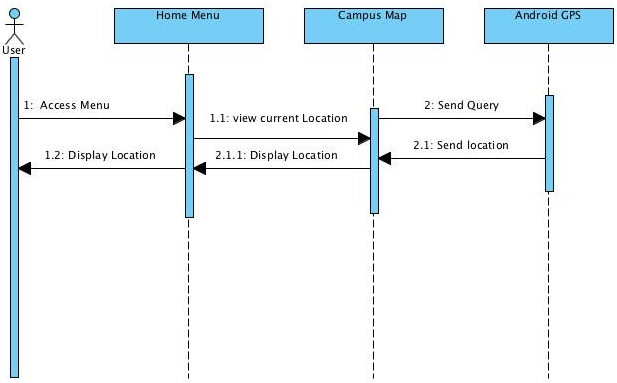
\includegraphics[keepaspectratio, scale=0.5]{seqfriend.png}
 \caption{View current location}
\end{figure}

\subsubsection*{Initial state}
The user already logs on the application and he is accessing the main menu
\subsubsection*{Normal action}
The user logs on the system. He clicks the button with the function to view location. The Map module sends query to the Android positioning server and a message containing user’s current location will be returned. The map module marks the position and represents it to the user.
\subsubsection*{Possibilities of failure}
The majority of the problem comes from the accuracy of the GPS. If the position where the user is at have good signals. There should not be a problem.
\subsubsection*{Complete state}
The user can see his current location marked on the map.

\section*{Appendix}

\includepdf{testplan.pdf}
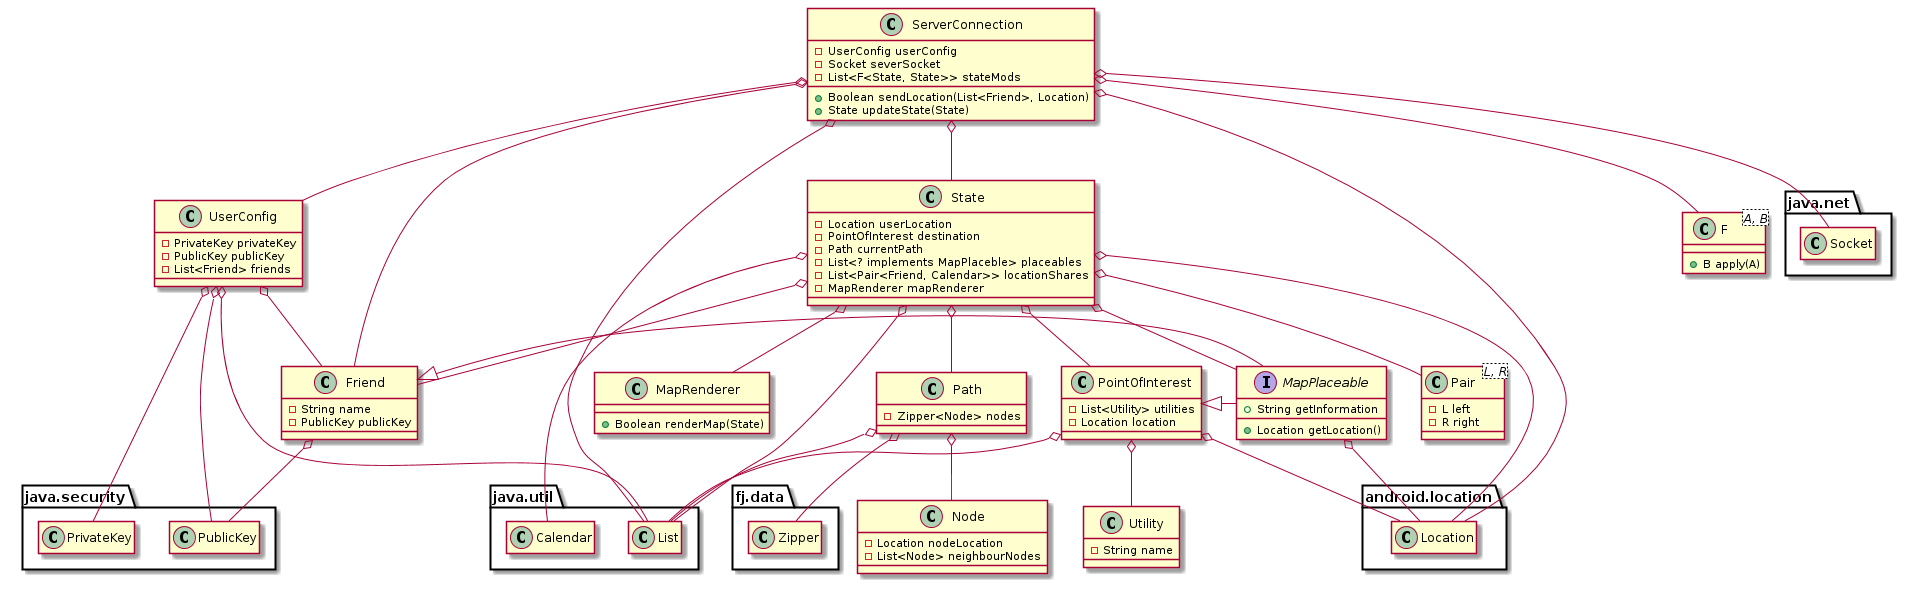
\includepdf[landscape=true]{class.pdf}

\end{document}
